%%%%%%%%%%%%%%%%%%%%%%%%%%%%%%%%%%%%%%%%%%%%%%%%%%%%%%%%%%%%%%%
%% HKUST Thesis LaTeX Template
%%
%% Check the project website for latest updates:
%% https://github.com/HKFoggyU/hkust-thesis
%%
%% Contributors:
%% https://github.com/HKFoggyU/hkust-thesis/graphs/contributors
%% 
%% License:
%% LaTeX Project Public License (version 1.3c)
%%
%%%%%%%%%%%%%%%%%%%%%%%%%%%%%%%%%%%%%%%%%%%%%%%%%%%%%%%%%%%%%%%

%% Pass options to loaded packages in `.cls` file:
% \PassOptionsToPackage{separate-uncertainty=true, separate-uncertainty-units=single}{siunitx}

%% The following option is to set hyperref colors for preview,
%% but commented by default for submission and printing
% \PassOptionsToPackage{colorlinks=true,urlcolor=blue,citecolor=red,anchorcolor=blue}{hyperref}

%% The following option is to display the full name of the authors.
%% It comes with the setting to display the full author names in the List of Publications
\PassOptionsToPackage{firstinits=false}{biblatex}

\documentclass[
  %customlatinfont = windows,
  %custombibstyle = nature,
  displaycommittee = false,
  blankpage = true,
]{hkustthesis}

%% Thesis information
\hkustsetup {
  %% Please wrap the items with {}.
  %% If one item is not applicable, just leave it {}.
  %% Please do not leave any blank lines without {}.
  info = {
    degree        = {mphil},  %% phd / mphil
    title         = {Algebraic Logic\texorpdfstring{\\}{}for Deep Learning},
    keywords      = {algebraic logic, deep learning, artificial intelligence},
    author        = {YKY},
    school        = {Some Univ in Canada},
    department    = {Department of Maths},
    program       = {Applied Mathematics},
    major         = {},
    supervisor    = {Prof. Who},
    %% Co-supervisor; leave it {} if not available
    co-supervisor = {Prof. Who Else},
    submit-month  = {August 2024},      % <month year>
    submit-date   = {13 August 2024},   % <date month year>
    defend-date   = {8 March 2024},     % <date month year>
    depthead      = {Prof. Ikari Someone, Head of Department},
    %% reviewers only for some departments, like ECE
    reviewer      = {Prof. AAA (Chairperson), 
                     Prof. BBB (Supervisor),
                     Prof. CCC (Co-Supervisor),
                     Prof. DDD,
                     Prof. EEE,
                     Prof. FFF},
    reviewerdept  = {Department of Electronic and Computer Engineering,
                     Department of ECE,
                     Department of ECE,
                     Department of ECE,
                     Department of ECE,
                     Department of Physics},
    reviewerext   = {Prof. FFF (External Examiner),
                     Department of HH\\{University of UU, at VV}},
    % reviewerext   = {},
    city          = {Hong Kong},
  }
}

%% Import extra packages
% \usepackage{indentfirst, xspace, xcolor}

%% Add custom command
% \newcommand{\todo}[1]{\textcolor{red}{TODO: #1}}
\newcommand{\eg}{\textit{e.g.}, }
\newcommand{\ie}{\textit{i.e.}, }

%% Import bib file for bibliography
\addbibresource{mythesis.bib}

\begin{document}

%% -------------------------------------------------
%% Thesis structure: In the order of
%% -------------------------------------------------
%% Titlepage  -> Authorization -> Signature ->
%% Acknowledgements ->
%% TOC -> List of Figures -> List of Tables ->
%% Abstract -> 
%% -------------------------------------------------
%% <Main body> -> 
%% -------------------------------------------------
%% References -> (Appendices)
%% -------------------------------------------------

\frontmatter
\maketitle 

\authorization
\signaturepage

\begin{acknowledgements}

Thank you, all the Evangelion.

\end{acknowledgements}


\tableofcontents
\listoffigures
\listoftables
% TODO: see \cmd{\newlistofalgorithms}
\newlistofalgorithms % This is to maintain the same appearance

%% Dedication and Preface are optional
%\begin{dedication}
  Dedicated to someone like you.
\end{dedication}

%\begin{preface}

Some preface text.

\begin{flushright}
Author\\
2021. HK
\end{flushright}

\end{preface}

\begin{abstract}

Some text.

\end{abstract}


%% -------------------------------------------------
%% Main body
%% -------------------------------------------------
\mainmatter

\chapter{Introduction}\label{chap:introduction}

\section{Background}

Lambek:
\begin{equation}
\begin{tikzcd}[row sep=1cm, column sep=0.6cm]
& \parbox{1.5cm}{\linespread{-0.5}\selectfont\centering type theory} \arrow[dl,dash] \arrow[dr,dash] & \\
\mbox{logic} \arrow[rr,dash] & {} & \parbox{1.5cm}{\linespread{-0.5}\selectfont\centering category theory}
\end{tikzcd}
\end{equation}

I am very curious to see if the two algebras below would coincide?
\begin{equation}
\begin{tikzcd}[row sep=1cm, column sep=0.6cm]
 & & \parbox{1.5cm}{\linespread{-0.5}\selectfont\centering type theory} \arrow[dl,dash] \arrow[dr,dash] & & & \\
\parbox{2cm}{\linespread{-0.5}\selectfont\centering algebraic logic} \arrow[rrrrr, dashed, dash, bend right] \arrow[r,dash] & \mbox{logic} \arrow[rr,dash] & {} & \parbox{1.5cm}{\linespread{-0.5}\selectfont\centering category theory} \arrow[r,dash] & \mbox{topos} \arrow[r,dash] & \parbox{2cm}{\linespread{-0.5}\selectfont\centering algebraic geometry}
\end{tikzcd}
\end{equation}

\section{Paul Halmos}

Every Boolean algebra $\mathbb{A}$ is isomorphic to the set of all continuous functions from $X$ into $\mathbb{O}$, where $X$ is the dual space of the algebra $\mathbb{A}$, and $\mathbb{O}$ is the Boolean algebra with 2 elements.  If there is a homomorphism $f$ between Boolean algebras $\mathbb{A} \rightarrow \mathbb{B}$ then there is a dual morphism $f^*$ between their dual spaces $Y \rightarrow X$:
\begin{equation}
\begin{tikzcd}[column sep=3cm, row sep=0.6cm]
\mathbb{A} \arrow[r,"f"] \arrow[d,shift left=2,phantom,"\cong"{anchor=south,rotate=90}] & \mathbb{B} \arrow[d,shift left=2,phantom,"\cong"{anchor=south,rotate=90}] \\
\overbracket{X} \arrow[d] & \overbracket{Y} \arrow[d] \arrow[l,"f^*"] \\
\underbracket{\mathbb{O}} & \underbracket{\mathbb{O}} 
\end{tikzcd}
\end{equation}

\section{The set-up}

The set of equations $F$ defines an algebraic set = \textbf{the world}:
\begin{equation}
F(x) = 0 .
\end{equation}
The objective of an intelligent agent is to learn $F$.

We have the function $f$ performing \textbf{prediction} of the immediate future:
\begin{equation}
\boxed{\mbox{current state}} \quad x_t \stackrel{f}{\mapsto} x_{t+1} \quad \boxed{\mbox{next state}} \;.
\end{equation}

In an infinitesimal sense, we can see $f$ as a \textbf{differential equation} describing the \textbf{world trajectory}:
\begin{equation}
\dot{x} = f(x) .
\end{equation}
So $F$ is the \textbf{solution} to this differential equation.

It seems that $F$ and $f$ are more or less equivalent ways to describe the world.

Logic can be turned into some form of algebra, and this algebra can be used to express either $F$ or $f$.  Perhaps both ways are feasible, or even mixing the two.

What does it mean to use logic to express $F$ or $f$?

The following table depicts the main correspondences relevant to our research:
\begin{equation}
\begin{tabular}{|c|c|c|}
	\hline
	\textbf{LOGIC} & \textbf{facts} & \textbf{rules} \\
		& \mbox{human(socrates)} & $\forall x. \mbox{human}(x) \rightarrow \mbox{mortal}(x)$ \\
	\hline
	\textbf{ALGEBRA} & \textbf{element} & \textbf{element} \\
		& $p \in \mathbb{A} $ & $(p \rightarrow q) \in \mathbb{A} $ \\
	\hline
	\textbf{WORLD} & \textbf{states} & \textbf{state transitions} \\
		& $x_t$ & $x_t \stackrel{f}{\mapsto} x_{t+1}$ \\
	\hline
\end{tabular}
\end{equation}
The relation between LOGIC and WORLD has been elucidated quite thoroughly in the AI literature.  Note that the state $x_t$ is made up of a set of facts (logic propositions).  A single step of logic inference results in a new conclusion $\delta x$ which is \textit{added} (as a set element) to the current state $x_t$ to form a new state $x_{t+1}$.  Here $t$ refers to ``mental time'' which does not necessarily coincide with real time.


\chapter{Example chapter}\label{chap:sample}

\section{Background}\label{chap:exp:sec:background}

\subsection{Cross references}

You can use \lstinline|\cref{}| to automatically setup the cross reference name; instead, you can always use \lstinline|\ref{}| to customize the appearance of the cross reference.

Chapter \ref{chap:introduction} tells you to read the latest PDF documentation.

\cref{chap:conclusions} is a conclusion.

\subsection{Citation and bibliography}

Use \lstinline|biber| as \hologo{BibTeX} backend.

Cite a book\cite{LaTeX.Companion}, some papers\cite{KeshavACMSIGCOMMComput.Commun.Rev.2007, WhitesidesAdv.Mater.2004}, and a conference\cite{, Babu2020IEEE33rdInt.Conf.MicroElectroMech.Syst.MEMS2020}.

\subsubsection{Citation database}

Bibliography entries (database) are stored in \lstinline|mythesis.bib|. You can use Zotero (or similar software) to generate \lstinline|another.bib| file. You can add multiple database files by adding their filenames one-by-one in the following commands in \lstinline|mythesis.tex|:

\begin{lstlisting}[language=TeX]
\addbibresource{mythesis.bib}
\addbibresource{another.bib}
\end{lstlisting}

\subsubsection{Citation style}

As described in the sample page from ECE department, the style is set to \lstinline|ieee| by default. You can modify the style in the \lstinline|hkustthesis.cls| file as you wish.

\section{Math}

\subsection{Symbols}

\begin{itemize}
  \item Calligraphic letters: $\mathcal{A}$
  \item Mathbb letters: $\mathbb{A}$
  \item Mathfrak letters: $\mathfrak{A}$
  \item Math Sans serif letters: $\mathsf{A}$
  \item Math bold letters: $\mathbf{A}$
  \item Math bold upright Greek letters: $\mathbf{\alpha}$ (Not displaying! Use the following one.)
  \item Math bold upright Greek letters: $\symbfup{\alpha}$
\item Math bold italic Greek letters\footnote{Avoid using \lstinline|bm| package as it conflicts with \lstinline|unicode-math| and it is outdated for \hologo{XeLaTeX}. You can alias some math commands by \lstinline|\\newcommand| or \lstinline|\\renewcommand| anyway.}: $\bm{\alpha}$
  \item Math bold italic Greek letters in upper case: $\mathbi{A}$
\end{itemize}

\subsection{Equations}

\begin{equation}
  E^2 = m^2 + p^2\label{eq:mass-energy}
\end{equation}

\cref{eq:mass-energy} or Equation (\ref{eq:mass-energy}) gives the mass-energy relationship.

\subsection{Theorem}

\begin{definition}
  LCL is orange juice.
\end{definition}

\begin{proof}
  They are both orange.
\end{proof}

\begin{algorithm}[htbp]
  \caption{Temp}
  \begin{algorithmic}[1]
    \STATE Temp
  \end{algorithmic}
\end{algorithm}

Available theorem environments are listed below:

algorithm, assumption, axiom, conclusion, condition, corollary, definition, example, lemma, proof, property, proposition, remark, theorem.

\section{Figure}
An example image is shown in \cref{fig:tikz example} or Figure (\ref{fig:tikz example}).

\begin{figure}[H]
  \centering
  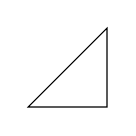
\begin{tikzpicture}
    \draw (0,0) -- (1, 0) -- (1, 1) -- cycle;
  \end{tikzpicture}
  \caption{An example tikz picture with a short caption.}
  \label{fig:tikz example short}
\end{figure}

\begin{figure}[H]
  \centering
  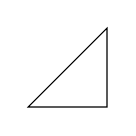
\begin{tikzpicture}
    \draw (0,0) -- (1, 0) -- (1, 1) -- cycle;
  \end{tikzpicture}
  \caption{An example tikz picture with breakline and\\ a very very very very very very very very very very very very very very very very very very very very very very very very very very very very very very very long caption.}
  \label{fig:tikz example}
\end{figure}

\section{Table}

An example table is shown in \cref{tab:environment} or Table (\ref{tab:environment}).

\begin{table}[H]
  \centering
  \caption{A table with a short caption.}
  \label{tab:table_short}
  \begin{tabular}{lll}
    \toprule
    OS           & TeX environment                & Test                                \\
    \midrule
    Overleaf     & \hologo{TeX}\,Live 2021$\sim$4 & Pass                                \\
    Windows 10   & \hologo{TeX}\,Live 2020        & \color{red}{\verb|ltxhook| problem} \\
    Ubuntu 20.04 & \hologo{TeX}\,Live 2021        & Pass                                \\
    \bottomrule
  \end{tabular}
\end{table}

\begin{table}[H]
  \centering
  \caption{Test result on different platforms with breakline and\\ a very very very very very very very very very very very very very very very very very very very very very very very very very very very very very very very long caption.}
  \label{tab:environment}
  \begin{tabular}{lll}
    \toprule
    OS                   & TeX environment                & Test                                \\
    \midrule
    Overleaf             & \hologo{TeX}\,Live 2021$\sim$4 & Pass                                \\
    Arch Linux (2024.10) & \hologo{TeX}\,Live             & Pass                                \\
    Windows 10/11        & \hologo{TeX}\,Live 2021        & Pass                                \\
    macOS 10.15          & \hologo{TeX}\,Live 2021        & Pass                                \\
    Windows 10           & \hologo{TeX}\,Live 2020        & \color{red}{\verb|ltxhook| problem} \\
    Ubuntu 20.04         & \hologo{TeX}\,Live 2021        & Pass                                \\
    Termux               & \hologo{TeX}\,Live 2021        & Pass                                \\
    Windows 11           & \hologo{MiKTeX} 4.9            & Pass                                \\
    Windows 10           & \hologo{MiKTeX} 4.4            & Pass                                \\
    \bottomrule
  \end{tabular}
\end{table}

\section{Code}

\subsection{Inline code}
Use \lstinline$\lstinline|<code>|$ to print code snippets. The \lstinline$||$ marks delimit
the code and can be replaced by any character not in the code;
\eg \lstinline|\lstinline$<code>$| gives the same result.

\subsection{Code environment}
The code to draw the \cref{fig:tikz example} is listed below:
\begin{lstlisting}[caption={\hologo{LaTeX} code for inserting a figure}]
\begin{figure}[htb]
  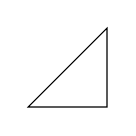
\begin{tikzpicture}
    \draw (0,0) -- (1, 0) -- (1, 1) -- cycle;
  \end{tikzpicture}
  \caption{An example picture with long caption: \blindtext\\\blindtext}
  \label{fig:tikz example} % this is a comment
\end{figure}
\end{lstlisting}

\chapter{Conclusions}\label{chap:conclusions}

Some conclusion text.


%% -------------------------------------------------
%% References
%% -------------------------------------------------

\printbibliography[heading=bibintoc,title=References]

%% -------------------------------------------------
%% Appendices
%% -------------------------------------------------
\appendix

\chapter{List of Publications}
% "List of Publications" citations can be stored in `mythesis.bib` or,
% another bib file, remember to add its name in `\addbibresource{}`

% Journal Publications
\paperlist[Journal Publications]{ChaiACSNano2022,HermanNature2007,WarrenSci.Adv.2022}

% Conference Publications
\paperlist[Conference Publications]{LuConf.LasersElectro-Opt.2021Pap.SW3B12021, JehleImagingAppl.Opt.20162016Pap.IM4F22016}

% You can add customized title name in the []

\chapter{FYTGS Requirements}
\label{chap:thesis-preparation}

The requirements are from the \href{https://rpghandbook.hkust.edu.hk/appendices-guidelines-on-thesis-preparation}{RPG Handbook}.

\section{Components}

\subsection{Order}

A thesis should contain the following parts in the order shown:

\begin{enumerate}
  \item Title page, containing in this order:
        \begin{enumerate}
          \item Thesis title
          \item Full name of the candidate
          \item Degree for which the thesis is submitted
          \item Name of the University, \emph{i.e.} The Hong Kong University of Science and Technology
          \item Month and year of submission
        \end{enumerate}
  \item Authorization page
  \item Signature page
  \item Acknowledgments
  \item Table of contents
  \item Lists of figures and tables
  \item Abstract ($\leq$ 300 words.)
  \item Thesis body
  \item Bibliography
  \item Appendices and other addenda, if any.
\end{enumerate}

\subsection{Authorization page}

On this page, students authorize the University to lend or reproduce the thesis.

\begin{enumerate}
  \item The copyright of the thesis as a literary work vests in its author (the student).
  \item The authorization gives HKUST Library a non-exclusive right to make it available for scholarly research.
\end{enumerate}

\subsection{Signature page}

This page provides signatures of the thesis supervisor(s) and Department Head confirming that the thesis is satisfactory.

\subsection{Acknowledgments}

The student is required to declare, in this section, the extent to which assistance has been given by his/her faculty and staff, fellow students, external bodies or others in the collection of materials and data, the design and construction of apparatus, the performance of experiments, the analysis of data, and the preparation of the thesis (including editorial help). In addition, it is appropriate to recognize the supervision and advice given by the thesis supervisor(s) and members of TSC.

\subsection{Abstract}

Every copy of the thesis must have an English abstract, being a concise summary of the thesis, in 300 words or less.

\subsection{Bibliography}

The list of sources and references used should be presented in a standard format appropriate to the discipline; formatting should be consistent throughout.

\textbf{Sample pages} of both MPhil and PhD theses are provided here (MPhil / PhD), with specific instructions for formatting page content (centering, spacing, etc.).

\section{Language, Style and Format}

\subsection{Language}

Theses should be written in English.

Students in the School of Humanities and Social Science who are pursuing research work in the areas of Chinese Studies, and who can demonstrate a need to use Chinese to write their theses should seek prior approval from the School via their thesis supervisor and the divisional head.

If approval is granted, students are also required to produce a translation of the title page, authorization page, signature page, table of contents and the abstract in English.

\subsection{Pagination}

\begin{enumerate}
  \item All pages, starting with the Title page should be numbered.
  \item All page numbers should be centered, at the bottom of each page.
  \item Page numbers of materials preceding the body of the text should be in small Roman numerals.
  \item Page numbers of the text, beginning with the first page of the first chapter and continuing through the bibliography, including any pages with tables, maps, figures, photographs, etc., and any subsequent appendices, should be in Arabic numerals.
  \item Start a new page after each chapter or section but not after a sub-section.
\end{enumerate}

\emph{Note: That means the Title page will be page i; the first page of the first chapter will be page 1.}

\subsection{Format}

\begin{enumerate}
  \item A conventional font, size 12-point, 10 to 12 characters per inch must be used.
  \item One-and-a-half line spacing should be used throughout the thesis, except for abstracts, indented quotations or footnotes where single line spacing may be used.
  \item All margins—top, bottom, sides—should be consistently 25mm (or no more than 30mm) in width. The same margin should be used throughout a thesis. Exceptionally, margins of a different size may be used when the nature of the thesis requires it.
\end{enumerate}

\subsection{Footnotes}

\begin{enumerate}
  \item Footnotes may be placed at the bottom of the page, at the end of each chapter or after the end of the thesis body.
  \item Like references, footnotes should be presented in a standard format appropriate to the discipline.
  \item Both the position and format of footnotes should be consistent throughout the thesis.
\end{enumerate}

\subsection{Appendices}

The format of each appended item should be consistent with the nature of that item, whether text, diagram, figure, etc., and should follow the guidelines for that item as listed here.

\subsection{Figures, Tables and Illustrations}

Figures, tables, graphs, etc., should be positioned according to the scientific publication conventions of the discipline, e.g., interspersed in text or collected at the end of chapters. Charts, graphs, maps, and tables that are larger than a standard page should be provided as appendices.

\subsection{Photographs/Images}

\begin{enumerate}
  \item High contrast photos should be used because they reproduce well. Photographs with a glossy finish and those with dark backgrounds should be avoided.
  \item Images should be dense enough to provide 300 ppi for printing and 72 dpi for viewing.
\end{enumerate}

\subsection{Additional Materials}

Raw files, datasets, media files, and high resolution photographs/images of any format can be included.

\emph{Note: Students should get approval from their department head before deviating from any of the above requirements concerning paper size, font, margins, etc. }


\end{document}
